\section{Data Analysis} \label{data}
The data is split into three main parts: \textit{demographics} (before playing the game), \textit{mid-questionnaire} (while playing the game) and \textit{post-questionnaire} (after playing the game). The mid-questionnaire consists of two parts. In the first part, participants described the game feel in their own words. In the second part, participants rated the game feel on pre-defined words using Likert scales. The post-questionnaire is about game feel in general. The following analyzes the data from the three parts.

\subsection{Demographics}
At the time of writing, 274 participants have played the game. The majority of the participants rated themselves very experienced with both videogames in general and 2D platformers. 70.6\% of the participants came from Europe and 26.7\% from USA. 93.6\% were male and 5.7\% female, with an average age of 24 years. Playing the game, the average death count per level was 5, the average framerate was 59.7 FPS and the average time spent per level was 61 seconds.

%\begin{table} \centering
%\small
%\caption{Demographical data 1.}
%\label{table:demographics1}
%\renewcommand{\arraystretch}{1.2}
%\begin{tabular}{cccc}
%\toprule
%\textbf{Platform} & Windows Web: & Windows Exe: & Mac Web: \\
%                  & 55.2\%      & 30.7\%      & 14.1\%  \\
%\textbf{Gender}   & Male:        & Female:      & Other:   \\
%                  & 93.6\%      & 5.7\%       & 0.7\%   \\
%\textbf{Age}      & Male:     & Female:            & Other:        \\
%                  & 24.6 years  & 23.9 years           & 25 years        \\
%\bottomrule
%\end{tabular}
%\end{table}

%\begin{table} \centering
%\small
%\caption{Demographical data 2.}
%\label{table:demographics2}
%%\renewcommand{\arraystretch}{1.2}
%\begin{tabular}{lcc}
%\toprule
%\textbf{Regions}                      &                & \textbf{}               \\ 
%\textit{Europe}                      & 70.6\%         &                         \\
%\textit{Americas}                    & 26.7\%         &                         \\
%\textit{Asia}                        & 1.9\%          &                         \\
%\textit{Oceania}                     & 0\%            &                         \\
%\textit{Africa}                      & 0.6\%          &                         \\
%\textit{Other}                       & 0.2\%          &                         \\
%\textbf{Experience with...} & \textbf{Videogames} & \textbf{2D platformers} \\
%\textit{1 (none)}                           & 0\%            & 0\%                     \\
%\textit{2}                           & 0\%            & 3.1\%                   \\ 
%\textit{3}                           & 0.6\%          & 10.1\%                  \\
%\textit{4}                           & 4\%            & 14.1\%                  \\ 
%\textit{5}                           & 9.6\%          & 23.2\%                  \\ 
%\textit{6}                           & 22.5\%         & 16.9\%                  \\
%\textit{7 (a lot)}                           & 63.3\%         & 32.6\%                  \\
%\bottomrule
%\end{tabular}
%\end{table}

Ideally, there should be an equal amount of participants in each of the four Latin square sequences. However, not all of the sequences received the same amount of participants. This might be due to players quitting halfway, presumably due to fatigue or boredom. Each time a participant collected three stars and answered the questionnaire, data was logged. In total, 701 data logs were collected.

Figure \ref{fig:overallDistribution} shows the overall distribution of the combinations of acceleration/deceleration time time that participants experienced. As stated previously, the time intervals were either \textit{fast} (1-240 ms) or \textit{slow} (241-1500 ms). Since the lengths of the two intervals are not of equal size, neither are the distribution, as shown in the figure. A way to counter this would be to divide the \textit{slow} category into multiple smaller intervals of equal sizes, but this would also affect the number of possible sequences and Latin squares.

%\begin{table} \centering
%\small
%\caption{The number of data entries in each of the four Latin square sequences.}
%\label{table:latinSequenceNumber}
%\begin{tabular}{cc}
%\toprule
%& \textbf{Number of data entries}\\
%\midrule
%\textbf{Sequence 1} & 190\\
%\textbf{Sequence 2} & 179\\
%\textbf{Sequence 3} & 165\\
%\textbf{Sequence 4} & 167\\
%\bottomrule
%\end{tabular}
%\end{table}

%\begin{figure}[htbp]
%\centering
%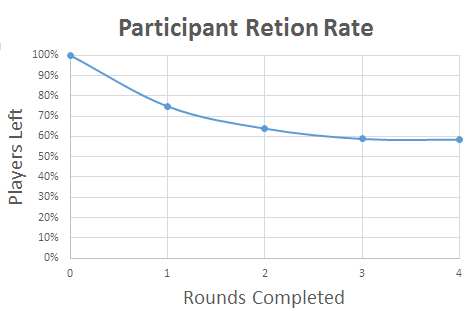
\includegraphics[width=0.4\textwidth]{Pics/retetionRate}
%\caption{274 participants started the game, but not all completed the four rounds, presumably due to %fatigue or boredom.}
%\label{fig:retention}
%\end{figure}

\begin{figure}[htbp]
\centering
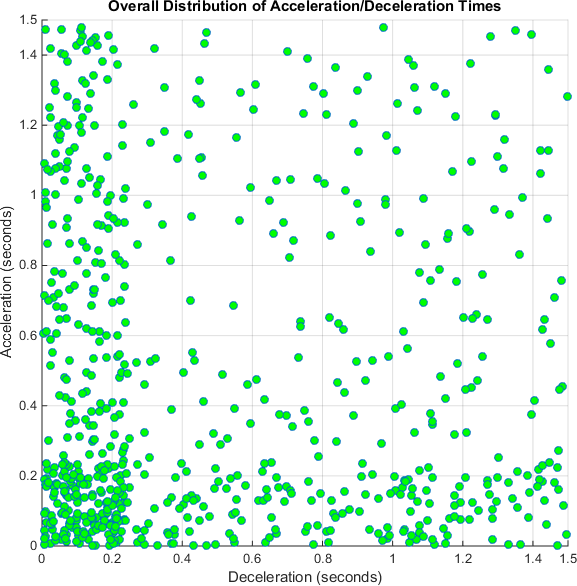
\includegraphics[width=0.55\columnwidth]{Pics/Classes/overall_distribution}
\caption{Scatter plot of all the different acceleration/deceleration combinations that participants experienced.}
\label{fig:overallDistribution}
\end{figure}

\subsection{Mid-questionnaire}
Whenever players collected three stars, they were met with a set of questions (see Figure \ref{fig:questionnaire}). In the first part, participants described the game feel in their own words, while in the second part they were asked to rate pre-defined words on a 7-point Likert scale (1 = \textit{not at all}; 7 = \textit{a lot}).

%\subsubsection{Describing Game Feel in Own Words}
%The game feel descriptions provided by the test participants have manually, by the author, been put into one or more of the following nine categories (see Figure \ref{fig:coding1}).
%\begin{itemize}[noitemsep,nolistsep]
%\item Single words or multiple words?
%\item Basic or complex words? (basic words are root words that can stand on their own, e.g., %\textit{heavy} and \textit{laggy}, whereas complex words consist of modifiers that somehow change the %meaning of the root words, e.g., \textit{very fast} and \textit{a bit sluggish})
%\item Did the words express anything about quality or opinion? (using words such as \textit{fun}, %\textit{too fast}, \textit{very annoying} and \textit{unrealistic})
%\item Did the words describe anything related to the difficulty?
%\item Did the words use physical properties or make comparisons to anything from the real world? %(\textit{like dragging through light mud}, using words such as \textit{force}, \textit{velocity} and %\textit{momentum})
%\item Did the words make comparisons to other games? (\textit{like Mario} or \textit{like Mega Man})
%\item Did the words make comparisons to previous rounds of the game? (\textit{felt no difference from %last game})
%\end{itemize}

%Note that a description can include words from multiple categories. The average word count was 5.4 words for ground descriptions and 5.1 words for air descriptions.

%Interestingly, there were some participants who had problems feeling any difference between the four rounds. One participant kept writing \textit{``No difference at all"}. This participant was presented with the following four sequences [acceleration;deceleration]: \textbf{[0.03;0.07]}, \textbf{[0.3;0.78]}, \textbf{[1.0;0.2]}, \textbf{[0.1;0.4]}. Assuming that the system worked correctly, it seems odd that the participant could not feel any difference between the rounds.

%Below are some selected quotes and their corresponding acceleration and deceleration values in square brackets (ascending order of acceleration values).
%\begin{itemize}[noitemsep,nolistsep]
%\item Grounded, wavy, skill-based, inertia, chunky. \textbf{[0.03;0.66]}
%\item It's okay fast. Not with an acceleration, just one constant speed (which maybe makes it easier %to control but then again more boring to look at). \textbf{[0.05;0.21]}
%\item Only goes where you want it to go. No physics. \textbf{[0.05;0.07]}
%\item Very responsive, felt ``right". \textbf{[0.06;0.03]}
%\item Icy. \textbf{[0.07;1.16]}
%\item Super twitchy, ball moves right when you press keys. \textbf{[0.09;0.14]}
%\item Annoying, no fine control, noticeable input delay. \textbf{[0.1;0.18]}
%\item Feels like you're rolling a big ball down a hill almost --- it takes a bit of time to get %going. \textbf{[0.27;1.47]}
%\item It feels really heavy and has a bit of after roll that adds a bit of reality feeling physics to %it. \textbf{[0.3;0.52]}
%\item Like Super Mario (which is good). \textbf{[0.34;0.14]}
%\item Heavy like a bowling ball, smooth. \textbf{[0.38;0.74]}
%\item Unrealistic, stiff. The fact that it stops on a dime, except when you press in the opposite direction feels odd. \textbf{[0.52;0.07]}
%\item The ball felt really good, and I liked that it didn't stop completely when I stopped pushing %the button. \textbf{[0.52;0.26]}
%\item BAD!!! Not like a ball at all. It is confusing. \textbf{[0.93;0.07]}
%\item Extremely annoying and heavy. Way too slow acceleration and reaction time in change of %direction was truly painful. \textbf{[0.97;0.29]}
%\item Slow, annoying, snappy. \textbf{[1.0;0.03]}
%\item Fast, but also slippery. \textbf{[1.06;1.17]}
%\item It controls like a truck with square wheels. \textbf{[1.19;0.07]}
%\item Lots of momentum, ball takes a while to accelerate and a while to decelerate. %\textbf{[1.22;1.29]}
%\item Very slow to start, stopped really fast. Punishing to not ``give full throttle". %\textbf{[1.24;0.09]}
%\item Mechanical, sometimes ``jumps" forwards. No fine control. \textbf{[1.3;1.1]}
%\item Sluggish, not fun. \textbf{[1.31;0.77]}
%\item Heavy and unpleasant as hell. \textbf{[1.41;0.02]}
%\item Felt like dragging through light mud with reasonable control. \textbf{[1.41;0.12]}
%\item Sticks like glue. \textbf{[1.47;0.01]}
%\end{itemize}

%Ostensibly, there are different opinions on what feels ``right". As one would expect, some of the higher values yield more frustrating results, since there is a longer delay before the participant sees the result on the screen. Some participants tried to describe the feeling using words from the physical world, such as \textit{momentum}, \textit{acceleration} and \textit{friction}. Others expressed themselves whenever they felt that the controls were \textit{too heavy} or \textit{too unresponsive}. Some compared it to \textit{a heavy tank moving through mud}, while others critiqued that the movement was \textit{unrealistic} and \textit{didn't feel like a ball at all}. Some participants were eager to express how much more \textit{difficult} or \textit{easier} the game was due to the controls, while others emphasized personal opinions, such as it feeling \textit{too fast} or \textit{not fun}.

%\begin{table} \centering
%\caption{The 30 most commonly-used words to describe the feel of the ball game. Numbers in %parenthesis indicate usage frequency. Common grammar words have been excluded.}
%\label{table:mostWords}
%\begin{tabular}{lll}
%\toprule
%heavy (165) & slow (132) & ball (122)\\
%responsive (104) & fast (94) & like (90)\\
%control (87) & very (83) & too (80)\\ 
%easy (78) & momentum (61) & realistic (61)\\
%sluggish (58) & floaty (58) & bit (54)\\
%air  (52) & good (51) & unrealistic (51)\\
%feels (50) & little (45) & hard (42)\\
%felt (40) & fluid (39) & still (38)\\
%ground (37) & jump (37) & same (36)\\
%speed (35) & time (34) & stop (31)\\
%\bottomrule
%\end{tabular}
%\end{table}

%\begin{figure}[htbp]
%\centering
%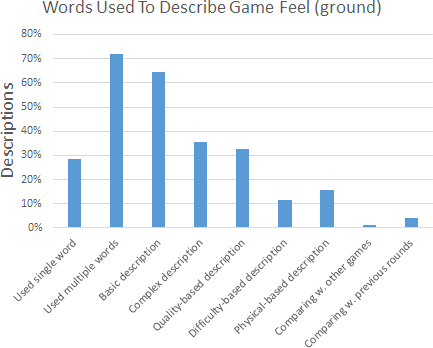
\includegraphics[width=0.8\columnwidth]{Pics/coding1}
%\caption{The different types of words participants used to describe the game feel on ground.}
%\label{fig:coding1}
%\end{figure}

%\begin{figure}[htbp]
%\centering
%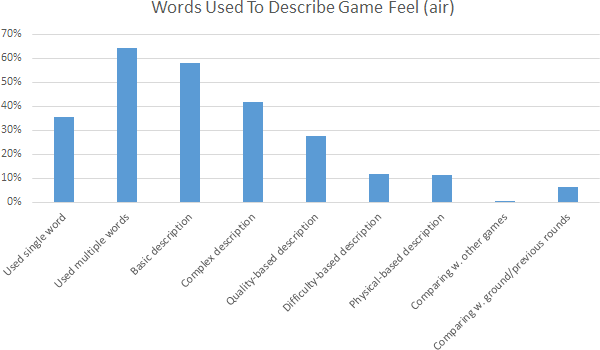
\includegraphics[width=\columnwidth]{Pics/coding2}
%\caption{The different types of words participants used to describe the game feel in air.}
%\label{fig:coding2}
%\end{figure}

%\begin{figure*}[htbp]
%\centering
%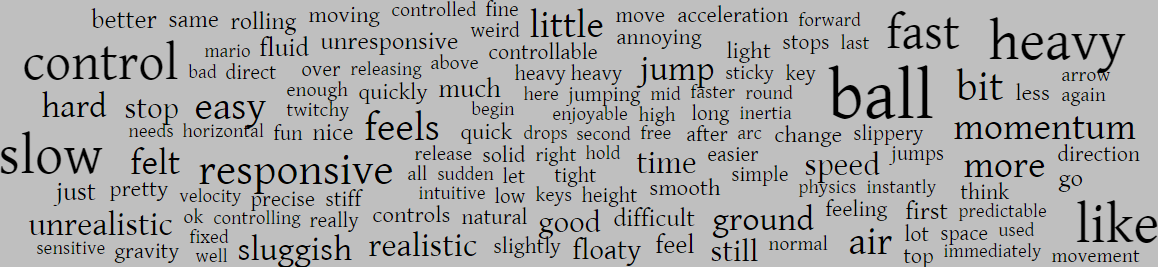
\includegraphics[width=1\textwidth]{Pics/wordcloud}
%\caption{The 130 most commonly-used words to describe the feel of the controls (both on ground and %in air). Bigger means a word has been used more frequently. Common words such as \textit{a}, %\textit{also}, \textit{and}, \textit{have}, \textit{could}, etc. have been excluded. Created with %WordItOut.com.}
%\label{fig:wordcloud}
%\end{figure*}

%\subsubsection{Rating Game Feel with Pre-Defined Words}
%Using a 7-point Likert scale, participants also rated the game feel on the following pre-defined terms: \textit{twitchy}, \textit{fluid}, \textit{stiff}, \textit{floaty}, \textit{responsive}, \textit{enjoyable}, \textit{difficult}, \textit{how much they liked the controls} and \textit{frustrated}.

%\subsubsection{Looking at Acceleration \& Deceleration Values Separately}
%Figure \ref{fig:correlationMatrix} shows the correlation matrix. Here, it is possible to spot a few tendencies, e.g., acceleration having a negative correlation with how \textit{twitchy}, \textit{fluid}, \textit{floaty} and \textit{responsive} the game felt. Meanwhile, deceleration has a positive correlation with how \textit{twitchy} and \textit{floaty} the game felt. However, this way of showing the data is not accurate, since it splits the acceleration and deceleration. The participants did not experience either separately; both were always apparent when playing.

%\begin{figure*}[htbp]
%\centering
%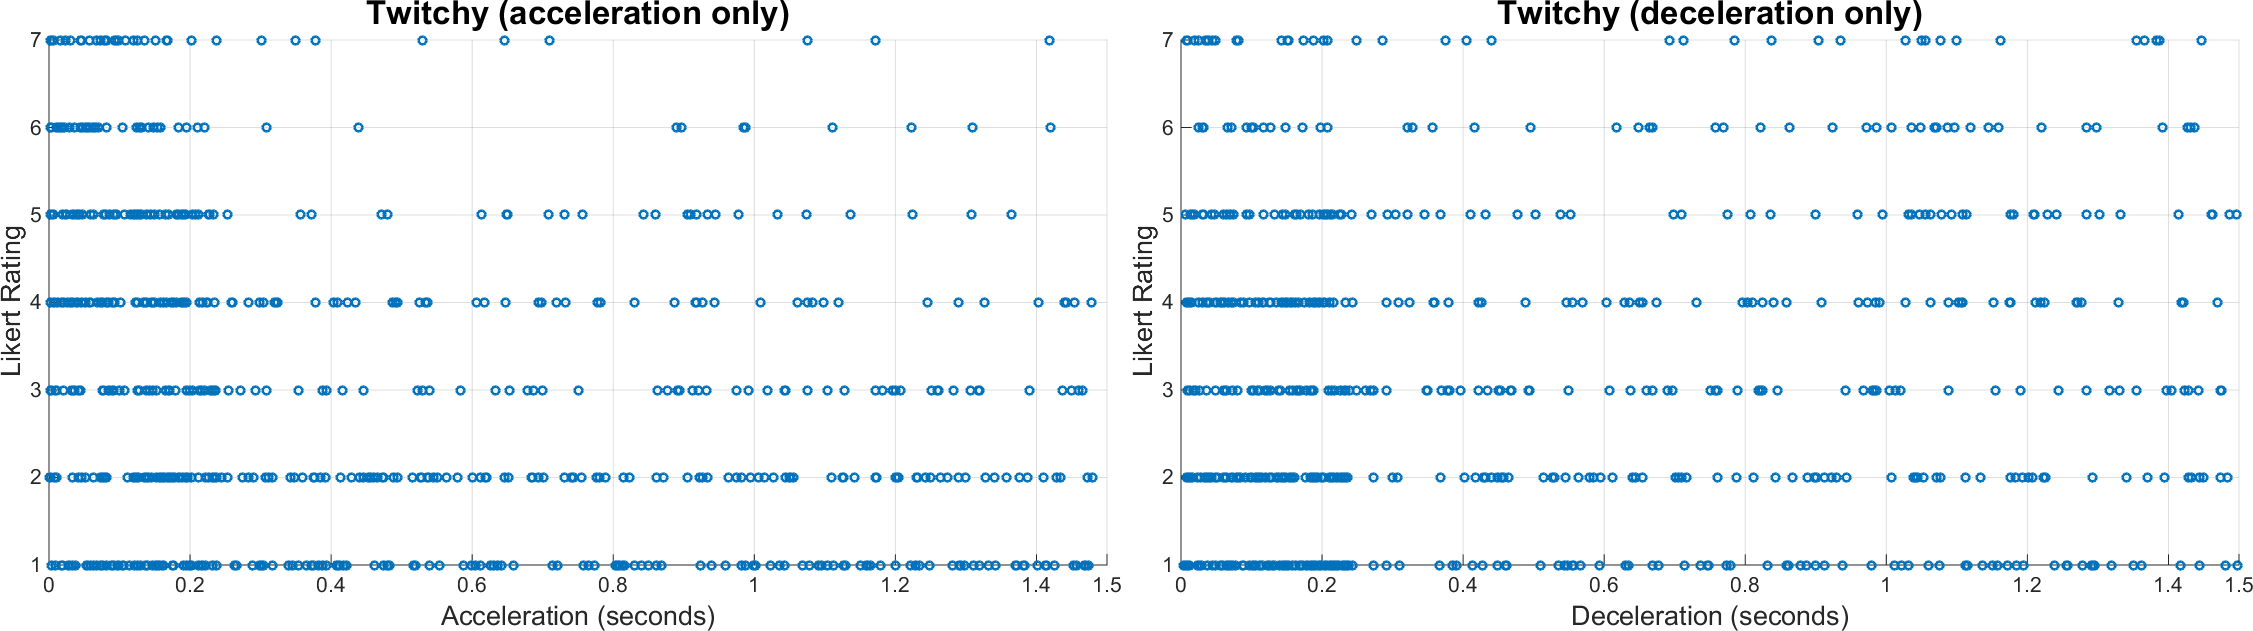
\includegraphics[width=0.95\textwidth]{Pics/Classes/twitchy_both}
%\caption{Looking at twitchy for acceleration and deceleration.}
%\label{fig:twitchy_both}
%\end{figure*}

%\begin{figure*}[htbp]
%\centering
%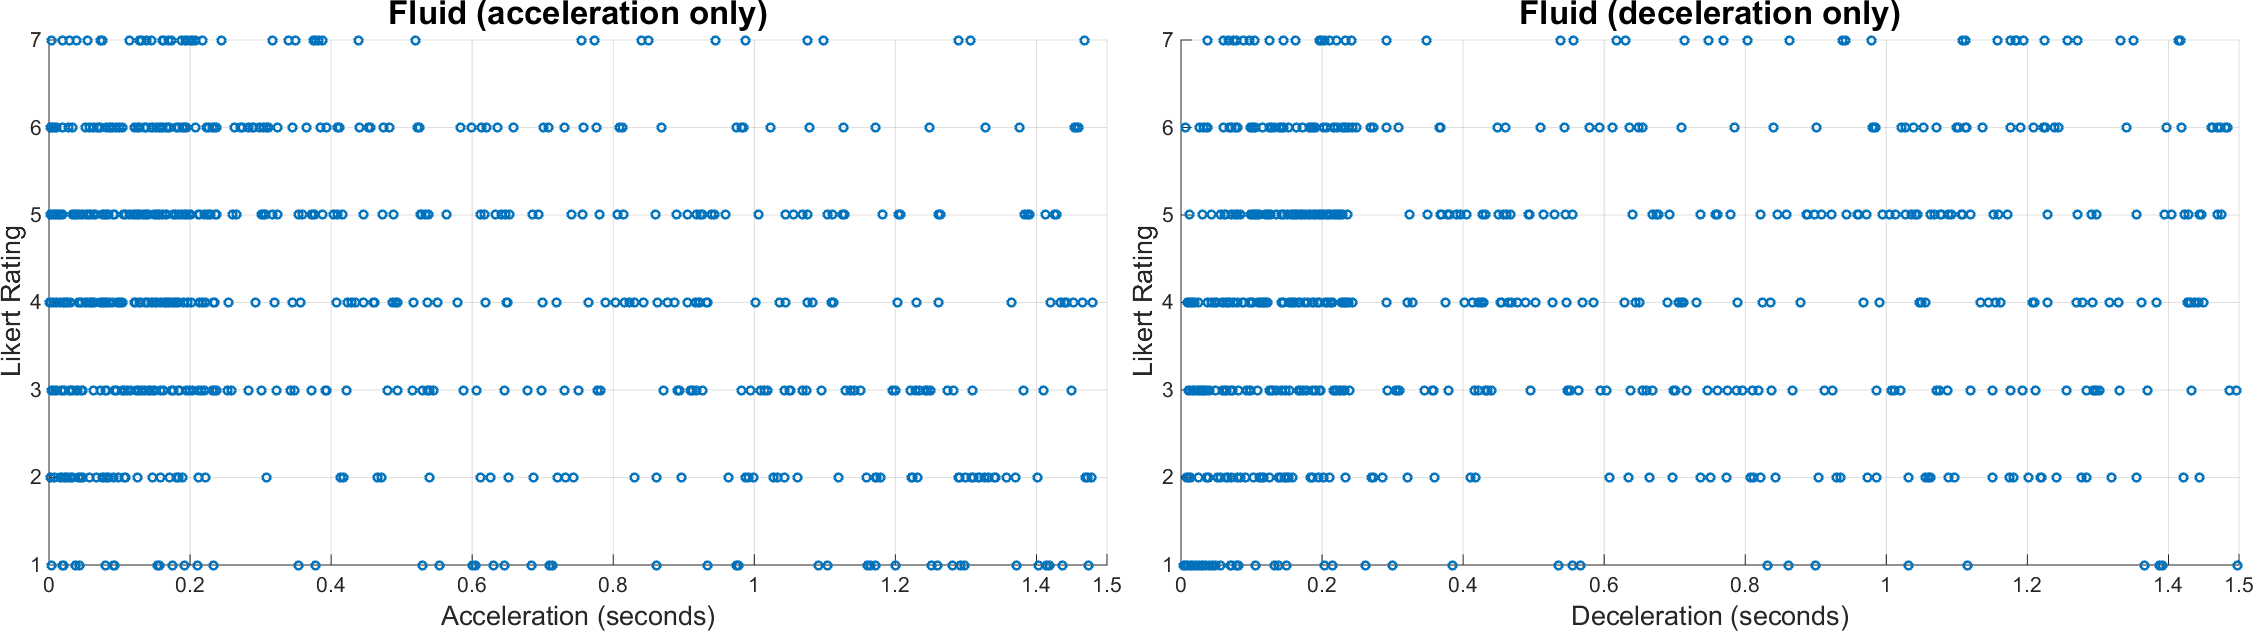
\includegraphics[width=0.95\textwidth]{Pics/Classes/fluid_both}
%\caption{Looking at fluid for acceleration and deceleration.}
%\label{fig:fluid_both}
%\end{figure*}

%\begin{figure*}[htbp]
%\centering
%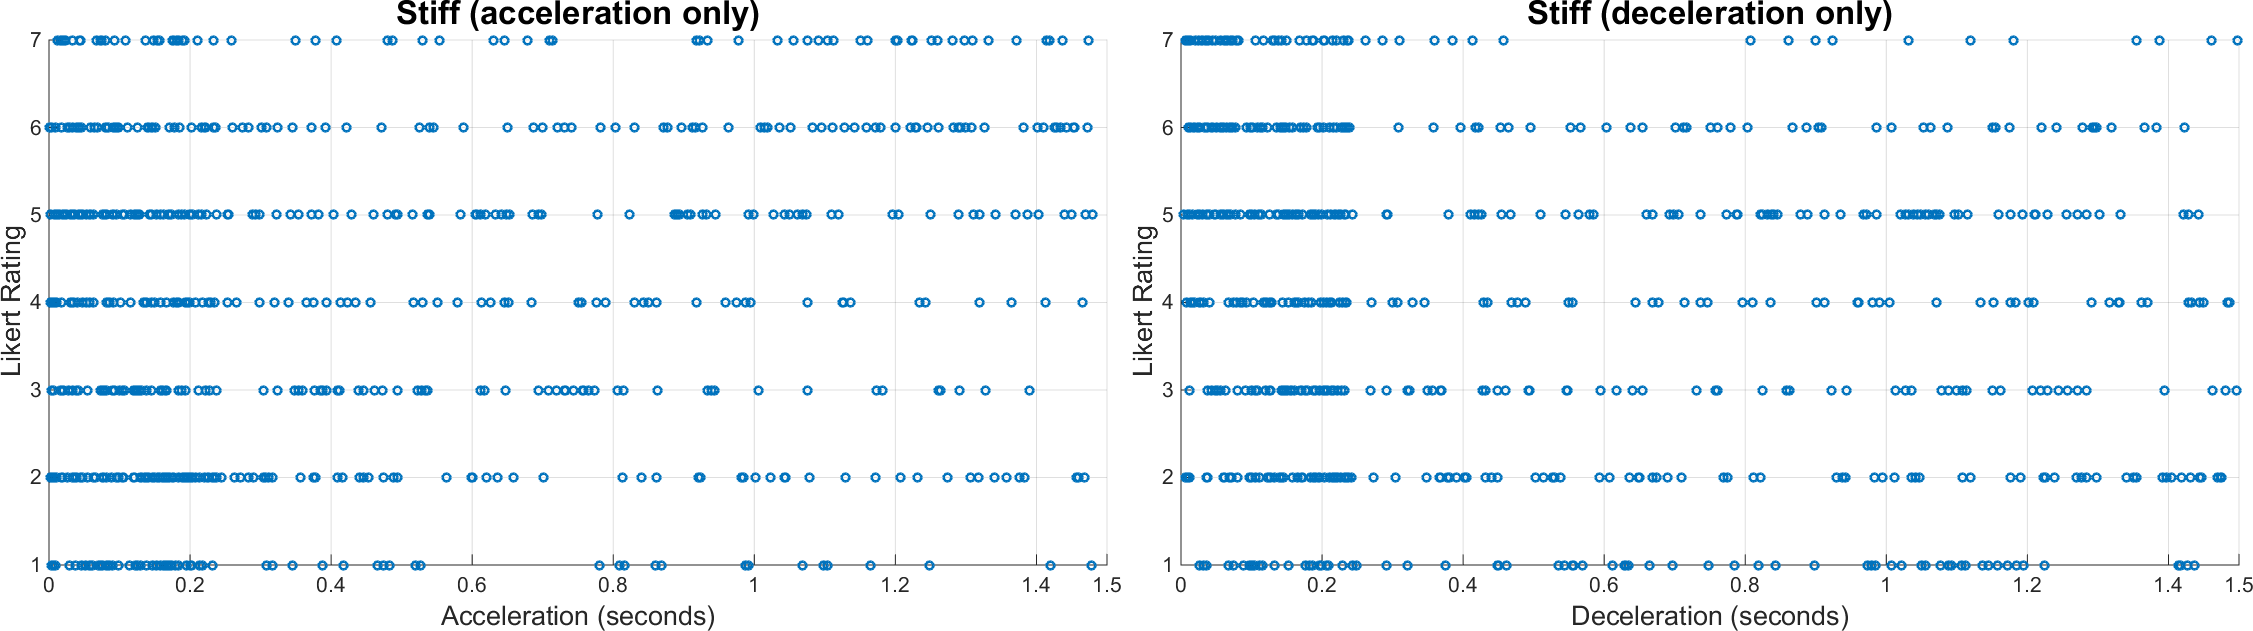
\includegraphics[width=0.95\textwidth]{Pics/Classes/stiff_both}
%\caption{Looking at stiff for acceleration and deceleration.}
%\label{fig:stiff_both}
%\end{figure*}

%\begin{figure*}[htbp]
%\centering
%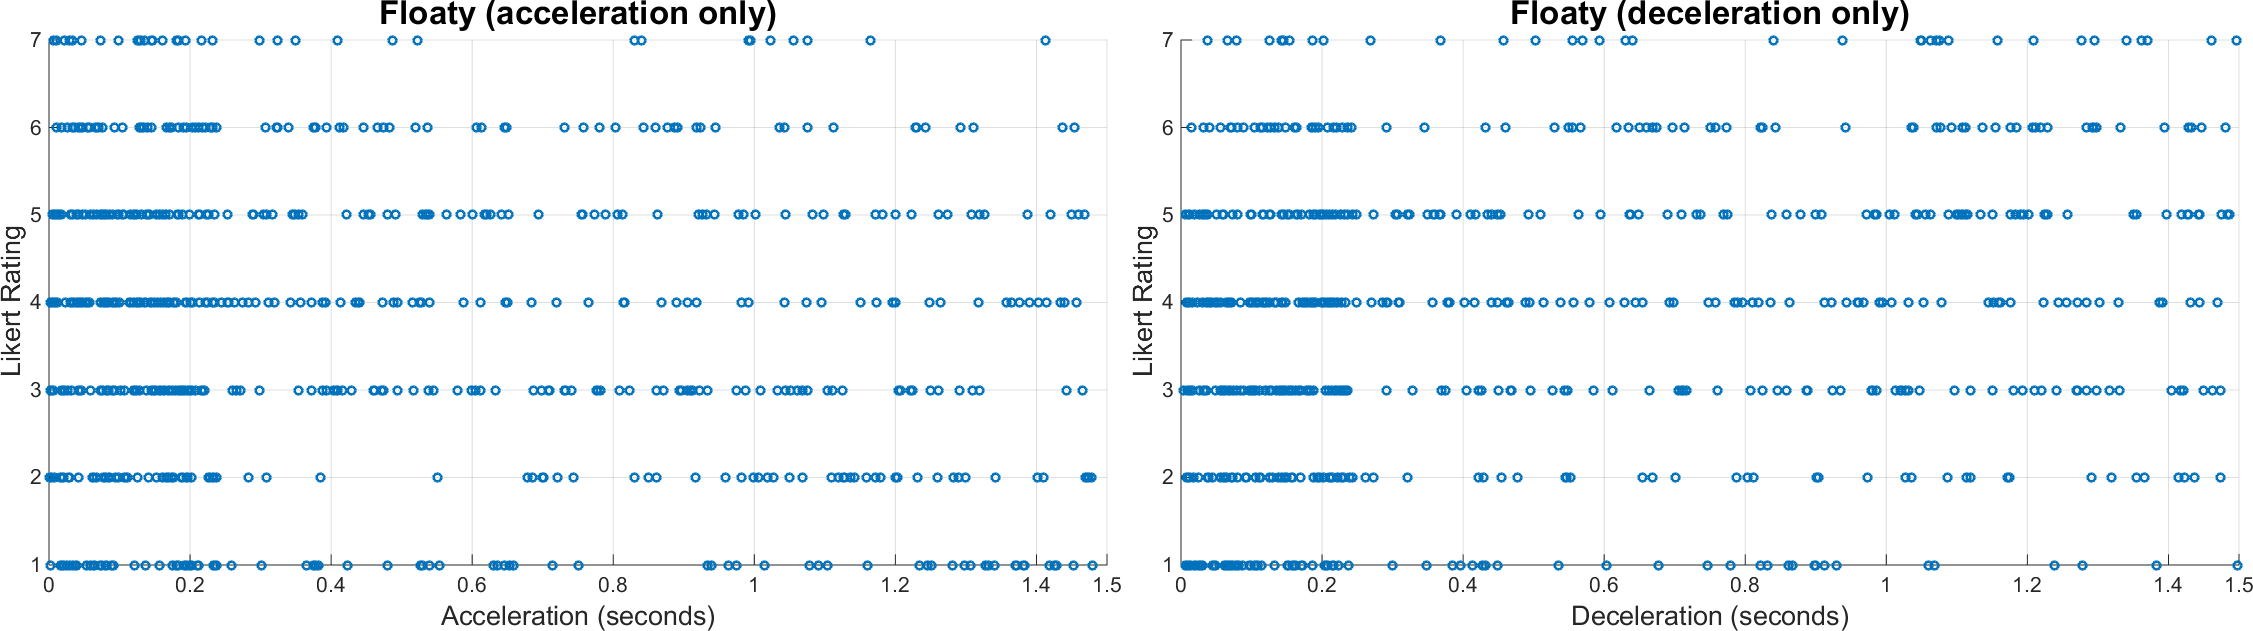
\includegraphics[width=0.95\textwidth]{Pics/Classes/floaty_both}
%\caption{Looking at floaty for acceleration and deceleration.}
%\label{fig:floaty_both}
%\end{figure*}

%\begin{figure*}[htbp]
%\centering
%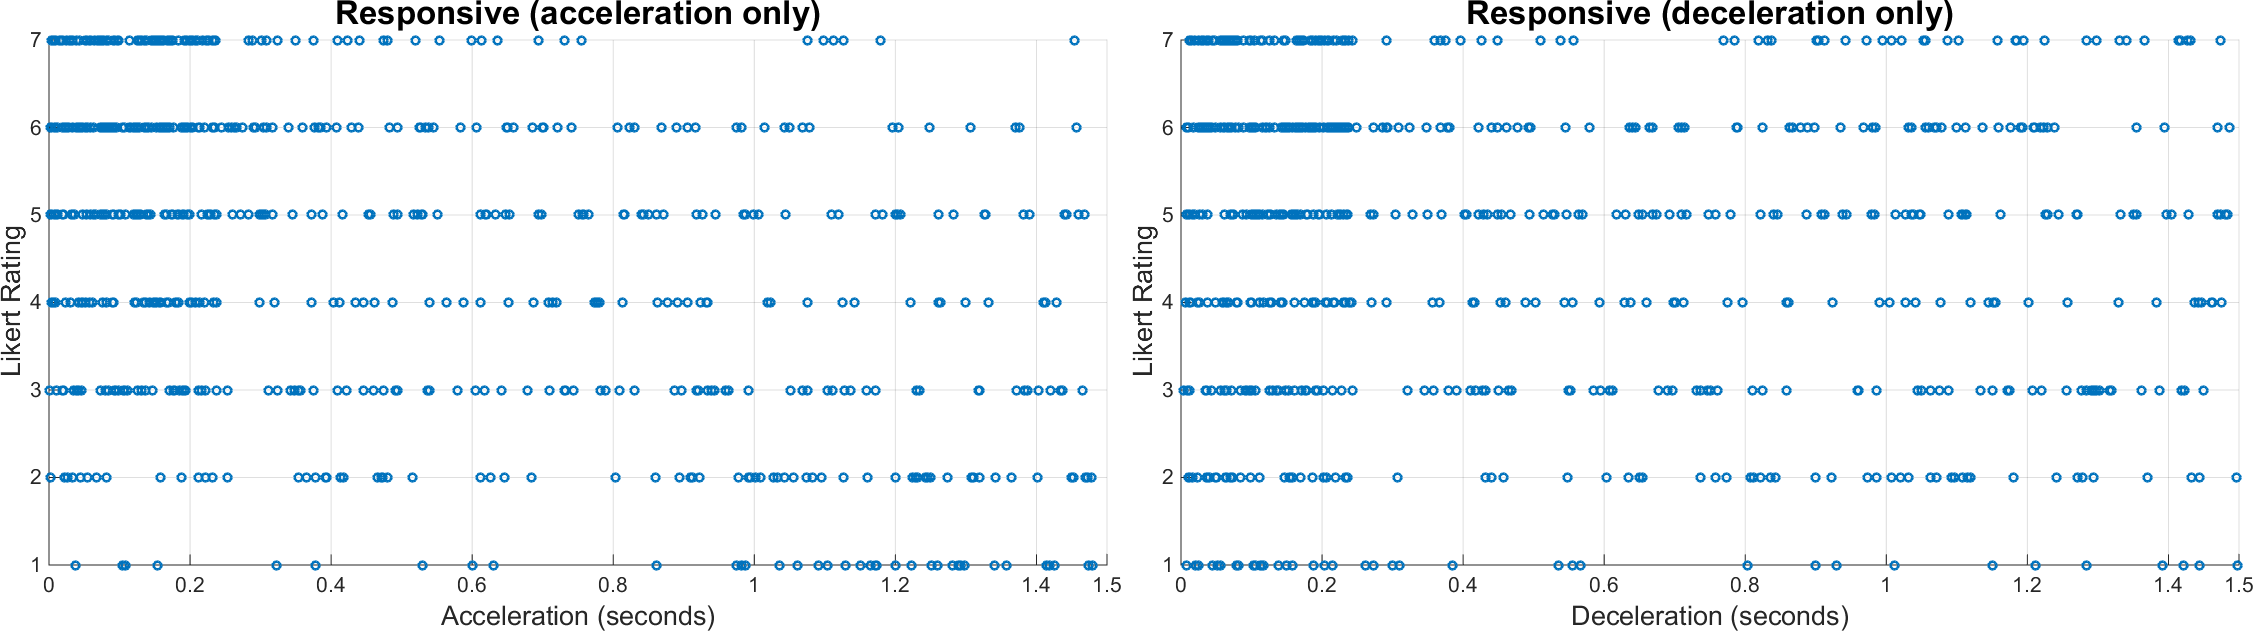
\includegraphics[width=0.95\textwidth]{Pics/Classes/responsive_both}
%\caption{Looking at responsive for acceleration and deceleration.}
%\label{fig:responsive_both}
%\end{figure*}

%\begin{figure}[htbp]
%\centering
%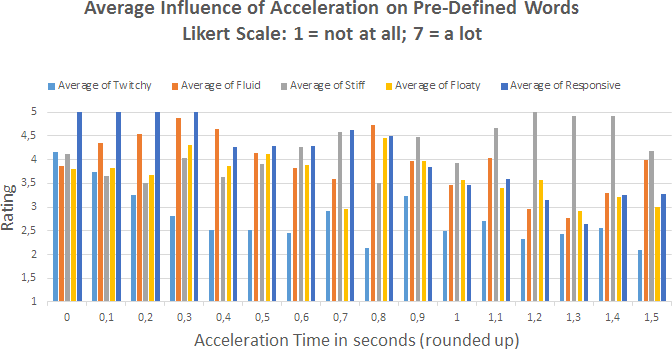
\includegraphics[width=0.97\columnwidth]{Pics/acc_average_response}
%\caption{Average ratings with acceleration.}
%\label{fig:acc_average_response}
%\end{figure}

%\begin{figure}[htbp]
%\centering
%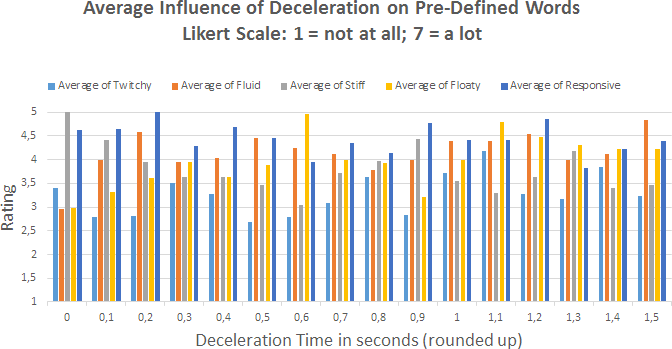
\includegraphics[width=0.97\columnwidth]{Pics/dec_average_response}
%\caption{Average ratings with deceleration.}
%\label{fig:dec_average_response}
%\end{figure}

\subsubsection{Rating Game Feel with Pre-Defined Words}
%\subsubsection{Looking at Acceleration \& Deceleration}
Since the distribution of the acceleration/deceleration times wasn't equal (due to the two intervals, \textit{fast} and \textit{slow}), one way to approach the data is to look at averages. In the following plots, the data has been divided into 36 boxes of size 0.25x0.25 seconds. The Likert ratings were counted for each of the boxes and then divided by the number of ratings in that particular box, resulting in an overall average.

It appears that the game felt most \textit{twitchy} with high acceleration times (> 1 second) and low deceleration times (< 0.25 seconds) (see Figure \ref{fig:twitchy_fluid_stiff_avg}). This might be due to the feeling of having slow acceleration, but when releasing the button, the avatar stops very suddenly.

Looking at Figure \ref{fig:twitchy_fluid_stiff_avg}, it seems like the game felt relatively fluid overall, especially with acceleration times above 0.75 seconds. However, with deceleration times above 1 seconds, it seems like the game feels less \textit{fluid}, even though the deceleration phase is longer and thus slower.

Considering the \textit{stiffness}, Figure \ref{fig:twitchy_fluid_stiff_avg} suggests that deceleration has a bigger influence. Times above 1 second resulted in the game feeling more \textit{stiff}. This can be understood in the sense that the avatar is slow to decelerate, or in other words, feels \textit{stiff} to move around.

The \textit{floaty} aspect seems to be influenced more by the acceleration, since times above 1 second yields a more \textit{floaty} feel (see Figure \ref{fig:floaty_responsive_enjoyable_avg}).

Figure \ref{fig:floaty_responsive_enjoyable_avg} depicts the \textit{responsiveness}. As already evident with the previously-shown quotes, low acceleration and deceleration generally makes the game feel more \textit{responsive}. It is interesting, though, that even if the acceleration times are relatively high, as long as the deceleration stays around 0.25 seconds, participants still reported the game to feel \textit{responsive}.

Looking at how \textit{enjoyable} (see Figure \ref{fig:floaty_responsive_enjoyable_avg}) and how much participants \textit{liked} the controls (see Figure \ref{fig:difficult_like_frustration_avg}), there don't appear any strong tendencies.

Lastly, Figure \ref{fig:difficult_like_frustration_avg} suggests that the game feels most \textit{difficult} and \textit{frustrating} with higher times in general, which is to be expected, since the time from input to feedback is longer and thus makes the avatar more difficult to control.

\begin{figure*}[!htb]
\centering
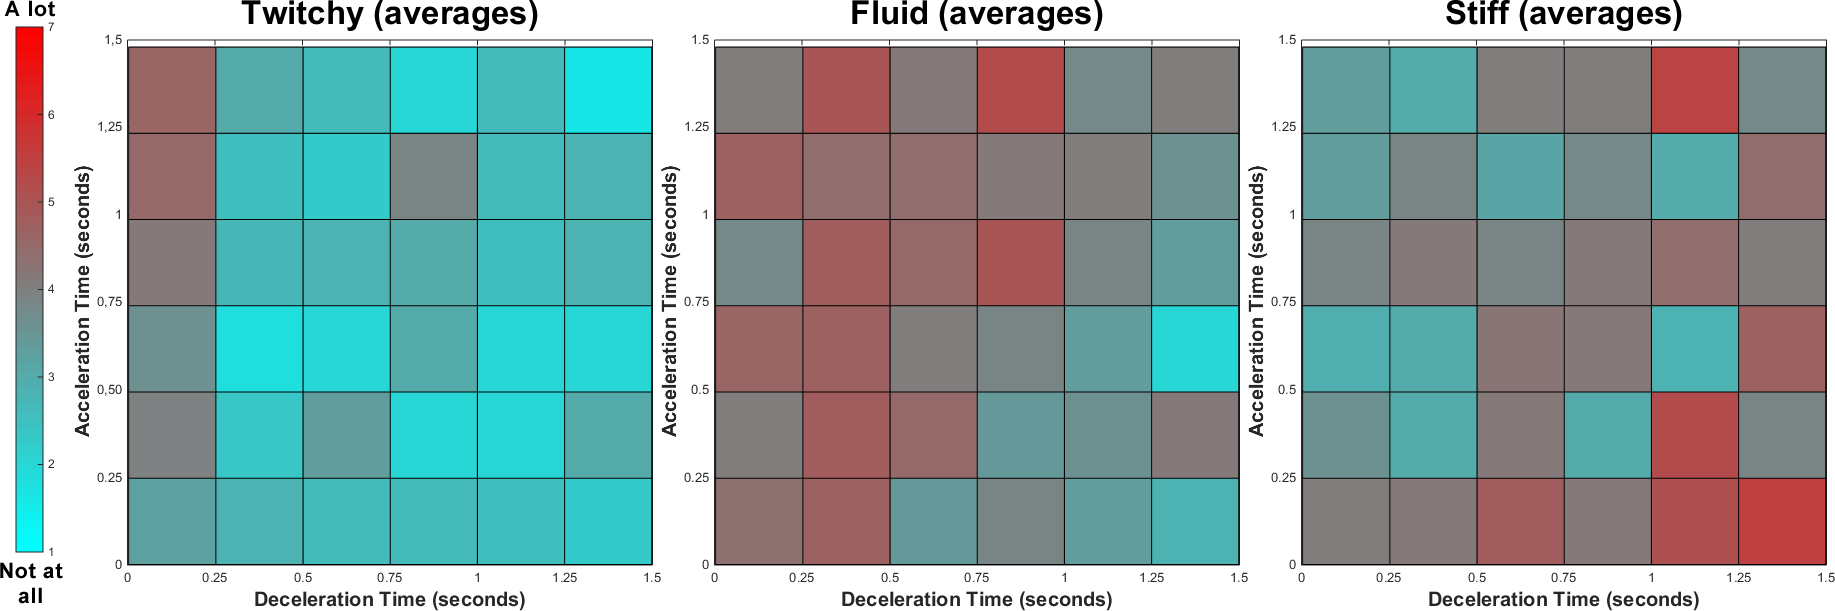
\includegraphics[width=0.97\textwidth]{Pics/Classes/averages/twitchy_fluid_stiff_avg}
\caption{Participants' average responses. Each box is 0.25x0.25 seconds.}
\label{fig:twitchy_fluid_stiff_avg}
\end{figure*}

\begin{figure*}[!htb]
\centering
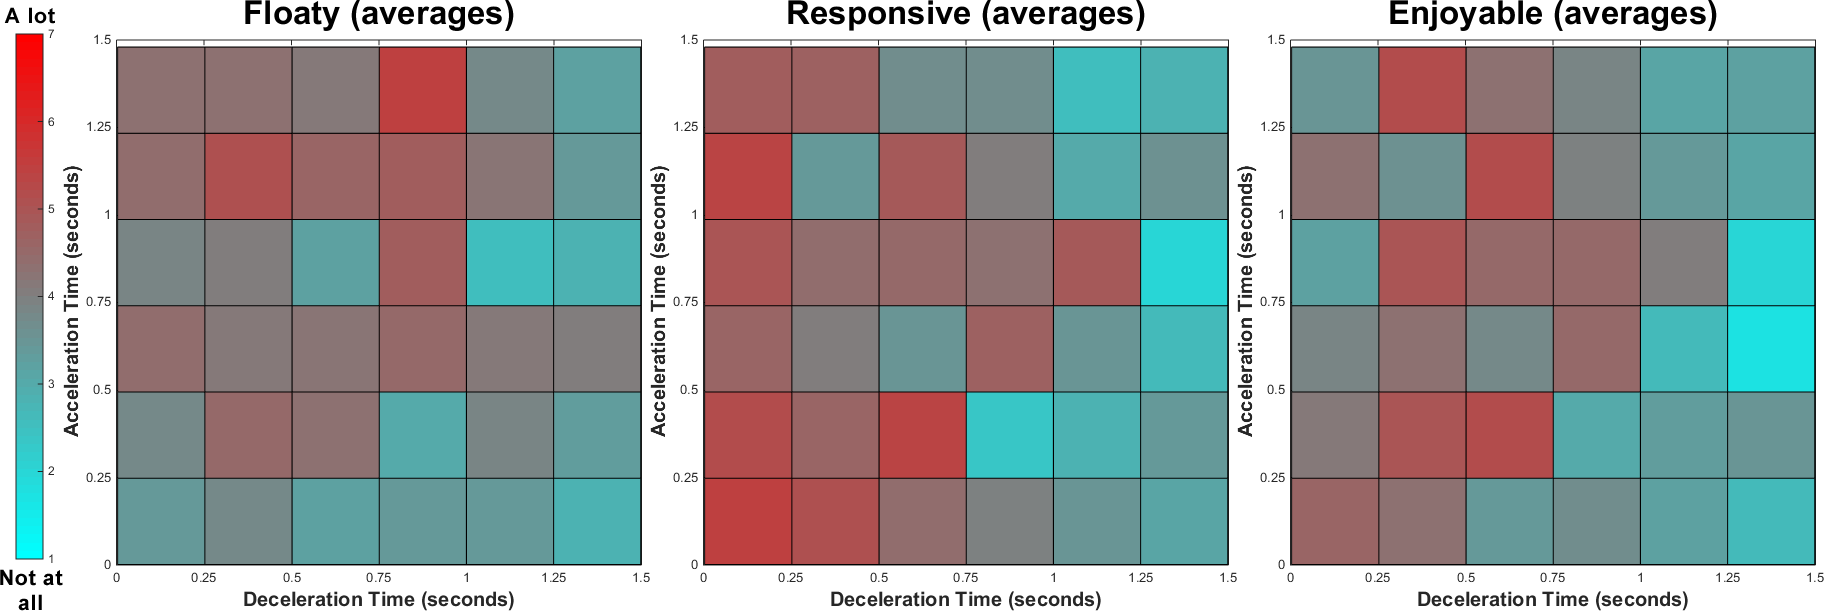
\includegraphics[width=0.97\textwidth]{Pics/Classes/averages/floaty_responsive_enjoyable_avg.png}
\caption{Participants' average responses. Each box is 0.25x0.25 seconds.}
\label{fig:floaty_responsive_enjoyable_avg}
\end{figure*}

\begin{figure*}[!htb]
\centering
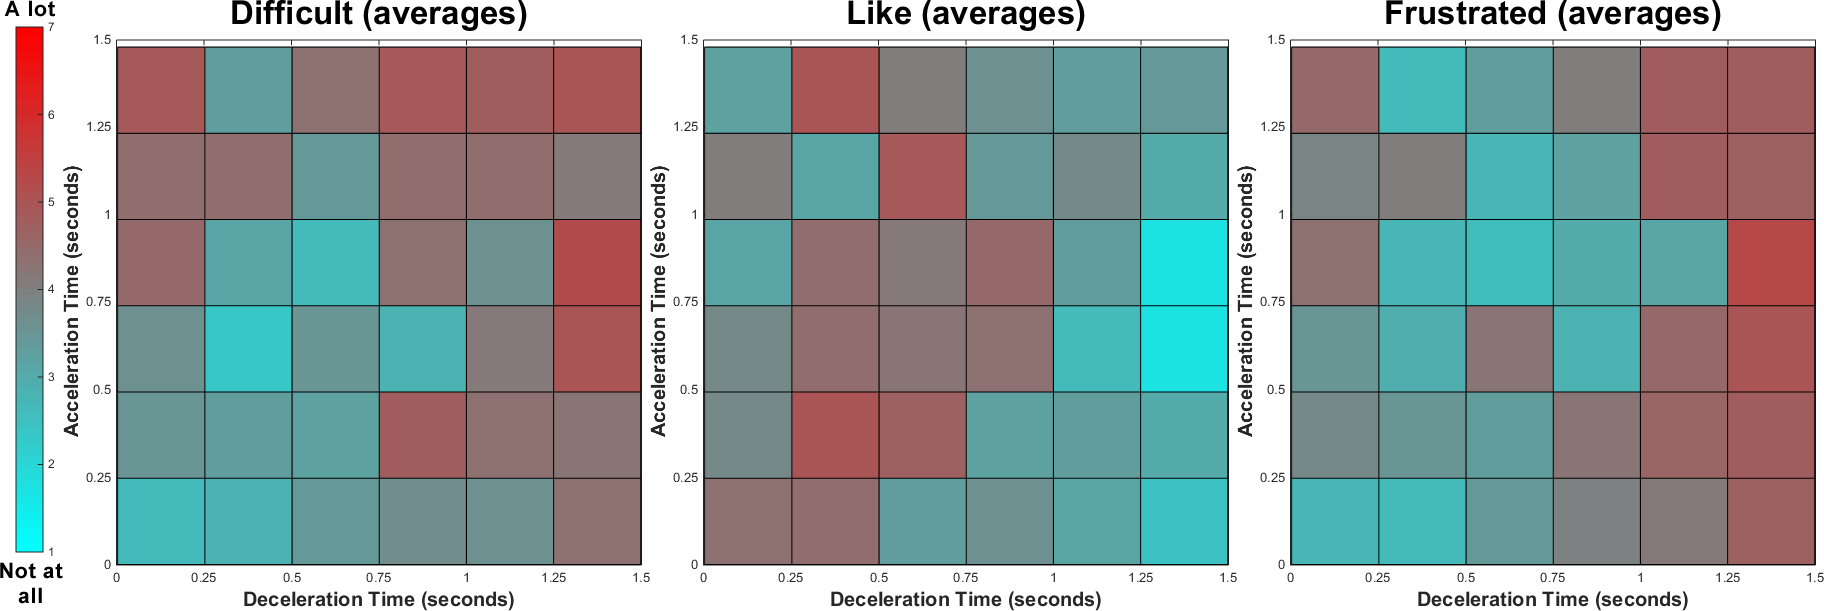
\includegraphics[width=0.97\textwidth]{Pics/Classes/averages/difficult_like_frustration_avg}
\caption{Participants' average responses. Each box is 0.25x0.25 seconds.}
\label{fig:difficult_like_frustration_avg}
\end{figure*}

%\begin{figure*}[htbp]
%\centering
%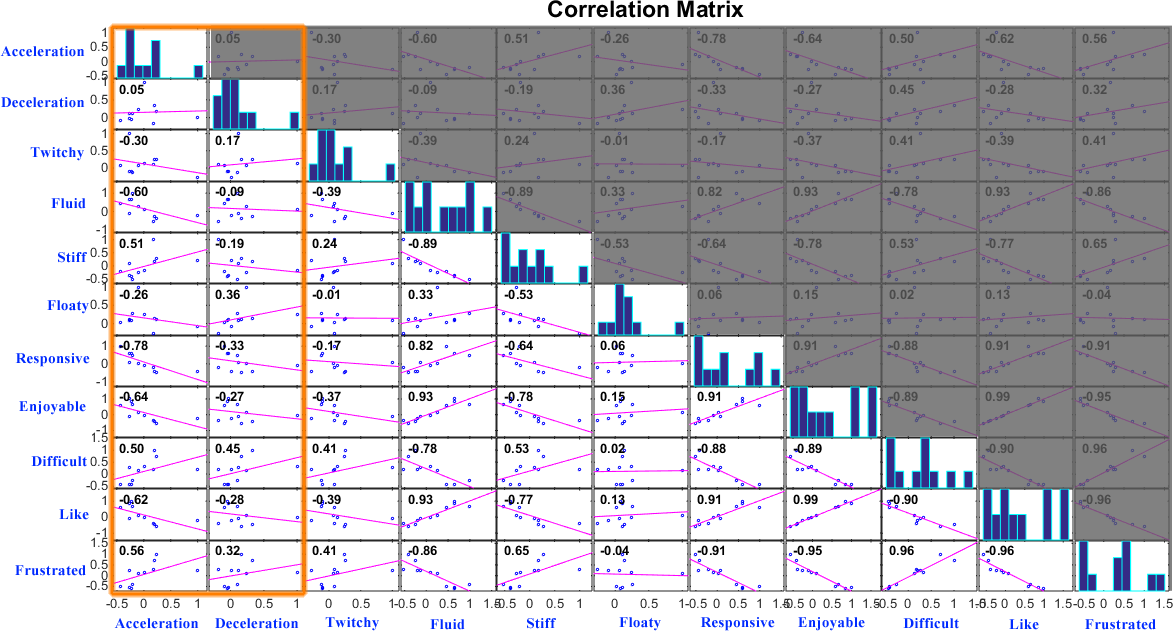
\includegraphics[width=0.98\textwidth]{Pics/correlationMatrix_final}
%\caption{Pearson correlation matrix.}
%\label{fig:correlationMatrix}
%\end{figure*}

%\subsubsection{Curves}
%Another way to visualize the data is to take the averages of the acceleration/deceleration values for each of the ratings, e.g., the average acceleration/deceleration values for \textit{twitchy} rating 1, rating 2, rating 3, etc. However, since a Likert scale consists of ordinal values, there is no guarantee that a rating difference of 1 represents an equal conceptual change, since the scale might be used differently by different participants. For instance, some participants might be hesitant to use the extreme values 1 (\textit{not at all}) and 7 (\textit{a lot}), while others might spread their answers across the whole scale \cite{cunningham}. Because of this, in the following graphs, the averages have been put into three weighted categories, so that the extreme ends contribute more. The \textit{low rating} curves consist of ratings 1 (70\%), 2 (20\%) and 3 (10\%). The \textit{mid rating} curves consist of ratings 3 (25\%), 4 (50\%) and 5 (25\%). The \textit{high rating} curves consist of ratings 5 (10\%), 6 (20\%) and 7 (70\%). Using these numbers, it is possible to draw acceleration/deceleration curves, as seen in Figures \ref{fig:twitchy_fluid}, \ref{fig:stiff_floaty}, \ref{fig:responsive_enjoyable} and \ref{fig:difficult_frustrated}. For all curves, the sustain time is 1 second. The numbers in square brackets represent acceleration and deceleration values.

%At first glance, many of the curves seem similar. However, when comparing the three curves from the same word, there are some differences. For instance, there is a difference of about 360 milliseconds between the deceleration in \textit{low rating} and \textit{high rating} in the \textit{floaty}. curve. Also, it should be noted that the different curves are not mutually exclusive, i.e., the controls can feel \textit{floaty} and \textit{fluid} at the same time.
%\begin{figure*}[!htb]
%\centering
%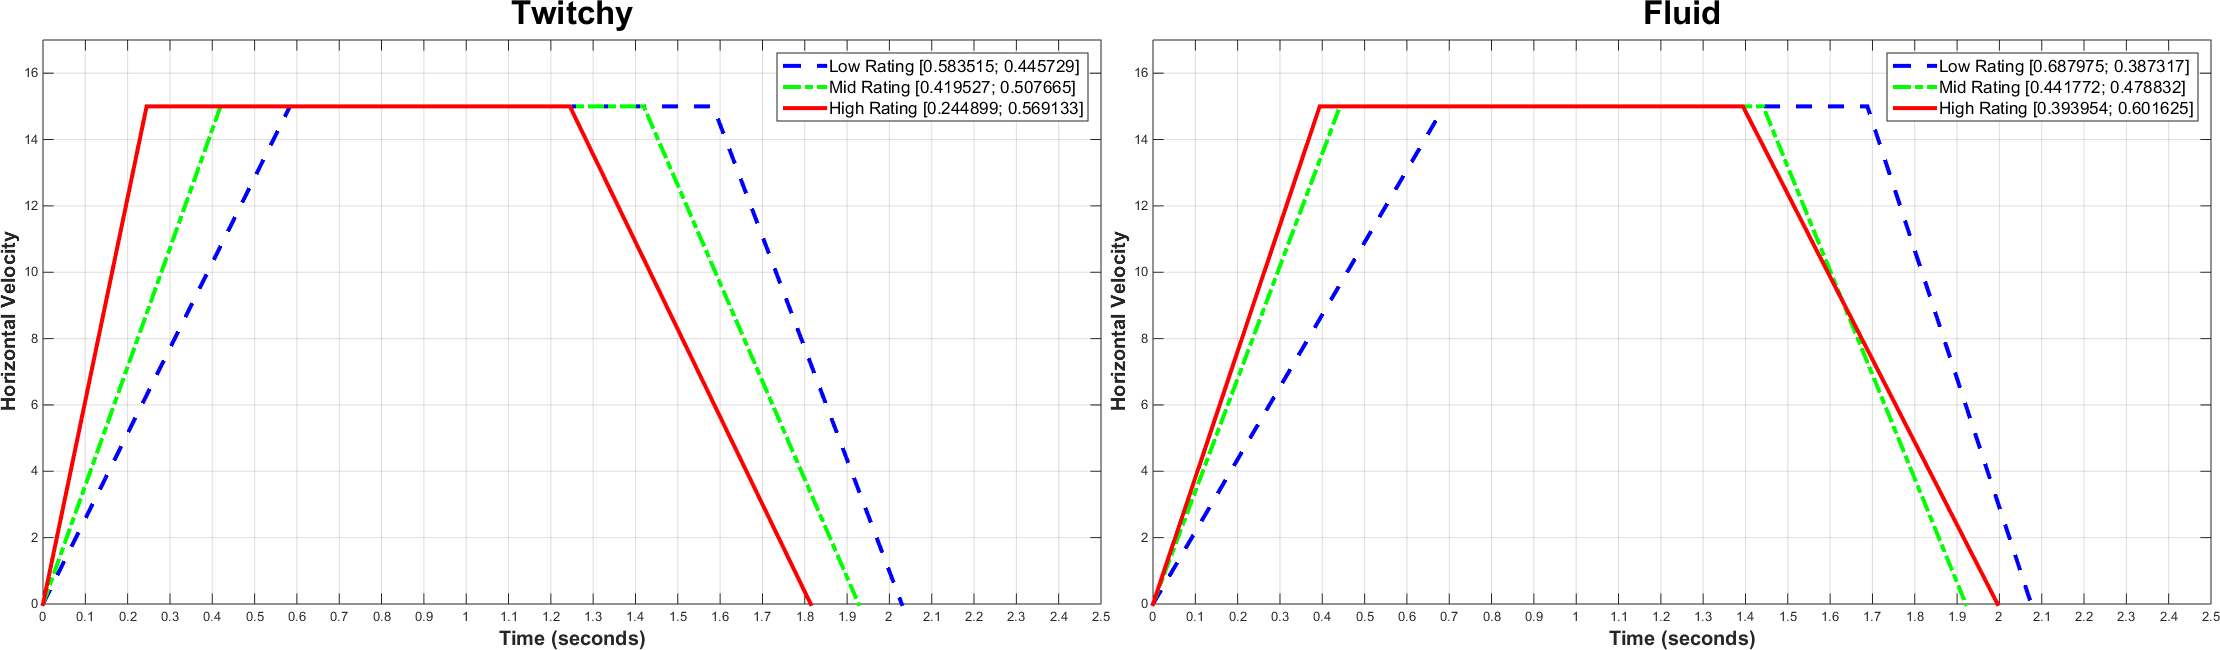
\includegraphics[width=0.97\textwidth]{Pics/Curves/twitchy_fluid}
%\caption{Twitchy and fluid curves.}
%\label{fig:twitchy_fluid}
%\end{figure*}

%\begin{figure*}[!htb]
%\centering
%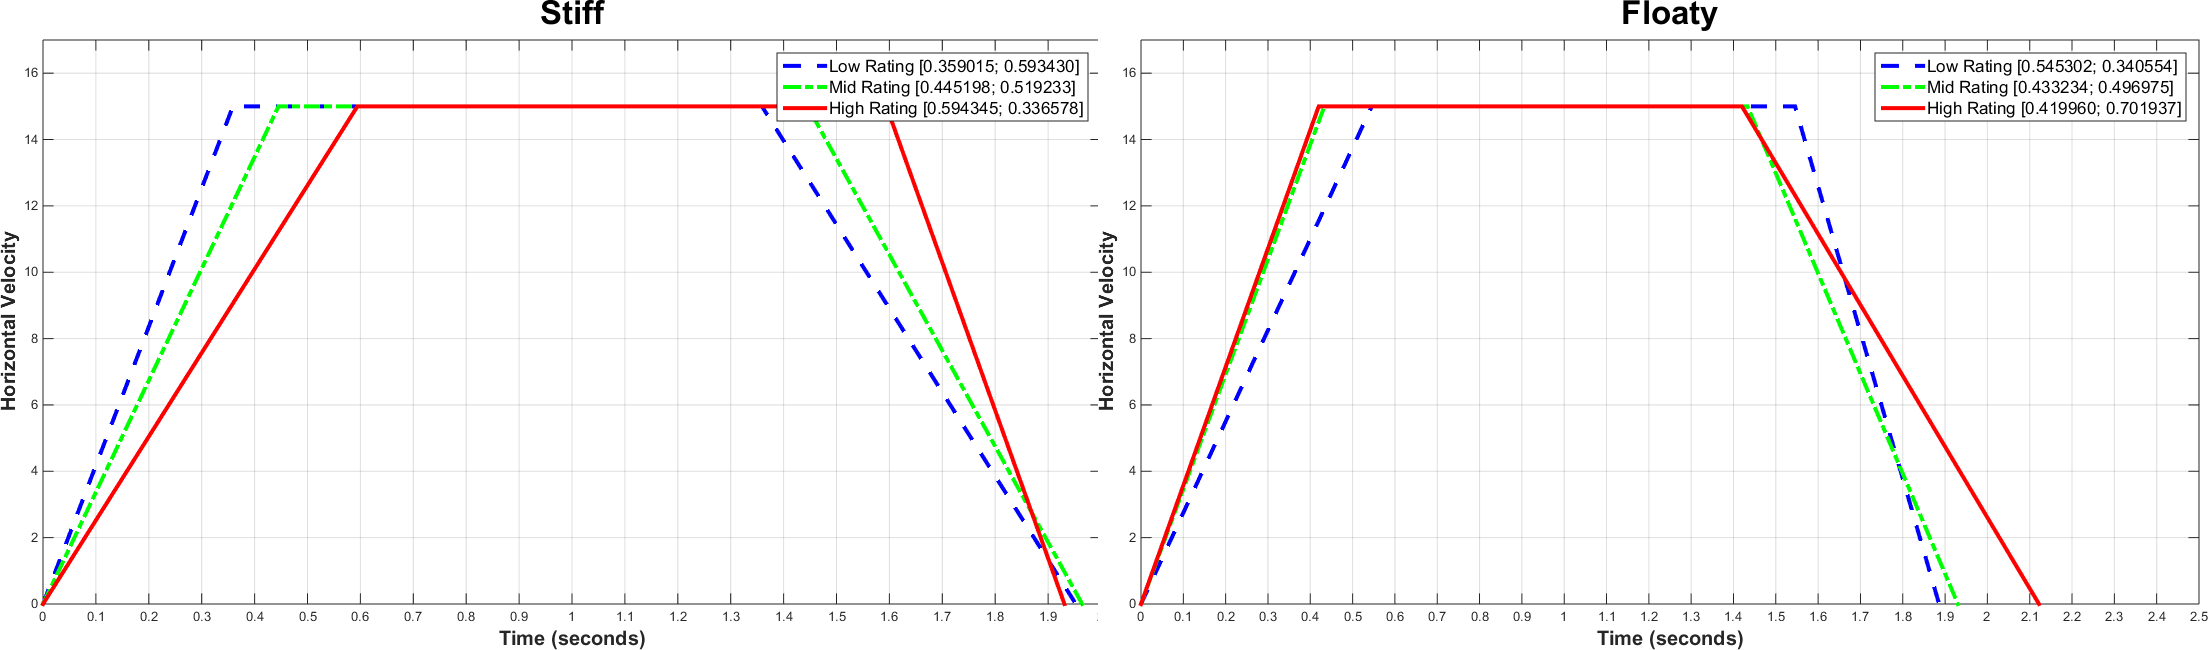
\includegraphics[width=0.97\textwidth]{Pics/Curves/stiff_floaty}
%\caption{Stiff and floaty curves.}
%\label{fig:stiff_floaty}
%\end{figure*}

%\begin{figure*}[!htb]
%\centering
%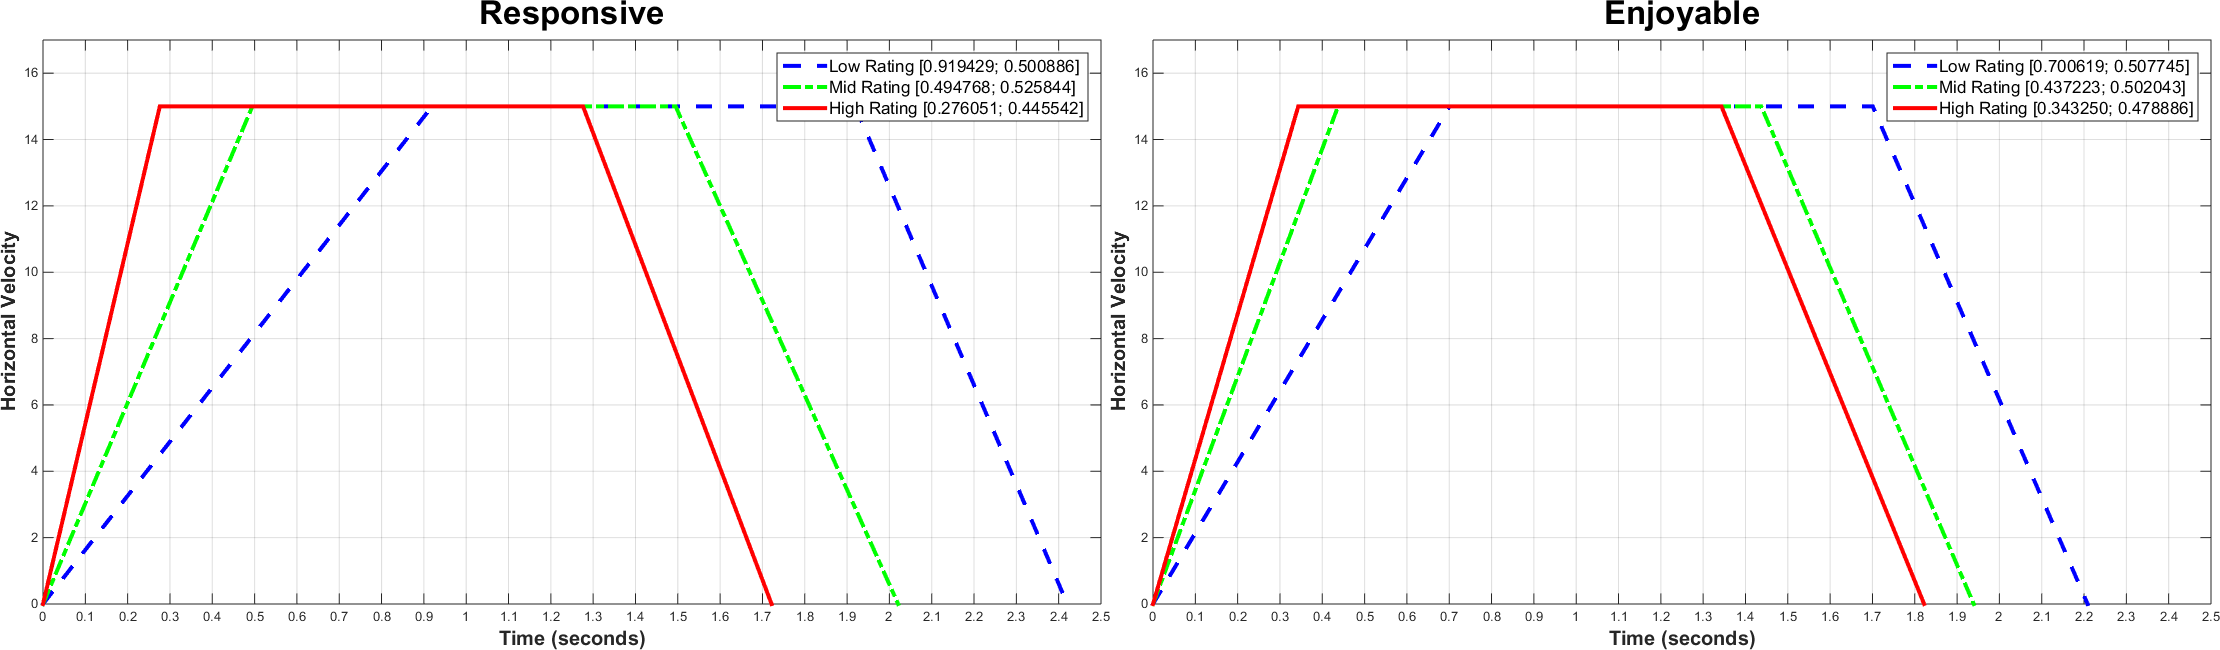
\includegraphics[width=0.97\textwidth]{Pics/Curves/responsive_enjoyable}
%\caption{Responsive and enjoyable curves.}
%\label{fig:responsive_enjoyable}
%\end{figure*}

%\begin{figure*}[!htb]
%\centering
%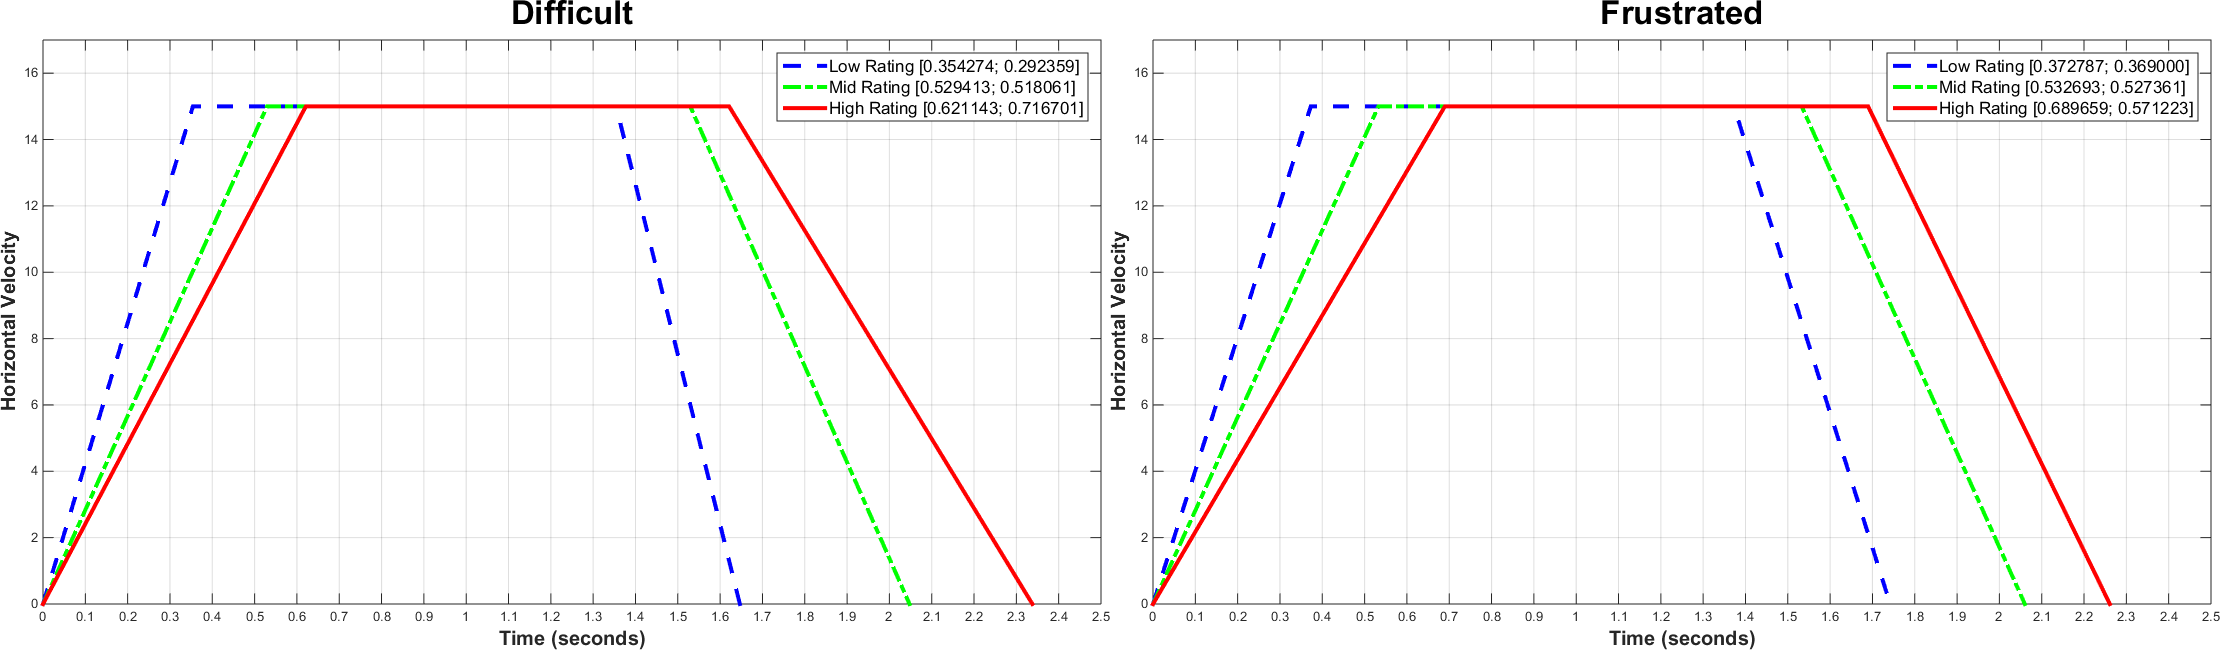
\includegraphics[width=0.97\textwidth]{Pics/Curves/difficult_frustrated}
%\caption{Difficult and frustrated curves.}
%\label{fig:difficult_frustrated}
%\end{figure*}

%\subsection{Post-questionnaire}
%After completing the fourth round of the game, participants were asked to complete a Google Forms questionnaire. At the time of writing, 153 participants have taken part in this post-questionnaire. Participants were asked to answer questions about what they thought changed between each round in the game. Even though only the acceleration and deceleration changed, the participants might have perceived more than this. Additionally, participants were asked to describe the feel of six commercially-released platforming games. This was to get a better understanding of how players describe game feel for platformers in general.

%\begin{figure*}[htbp]
%\centering
%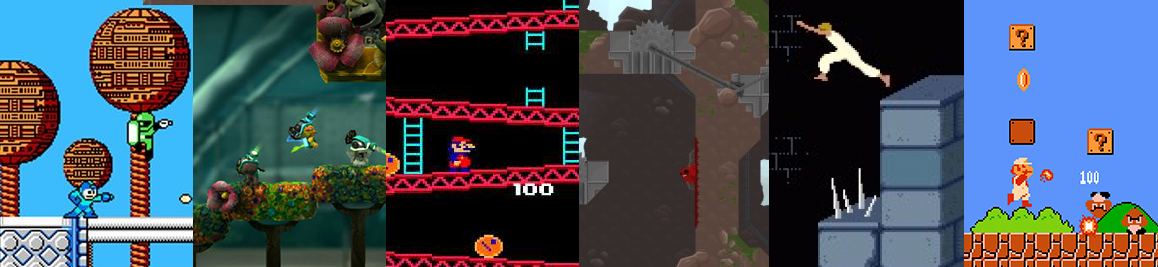
\includegraphics[width=1\textwidth]{Pics/rate_games_all}
%\caption{Participants described the feel of six platforming games. From left to right: \textit{Mega %Man}, \textit{LittleBigPlanet}, \textit{Donkey Kong}, \textit{Super Meat Boy}, \textit{Prince of %Persia} and \textit{Super Mario Bros.}}
%\label{fig:rate_games_all}
%\end{figure*}

%\begin{figure}[htbp]
%\centering
%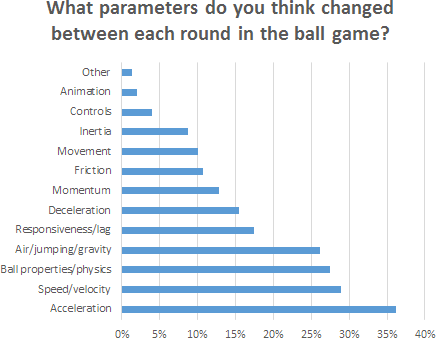
\includegraphics[width=0.9\columnwidth]{Pics/whatChanged}
%\caption{What the participants thought changed between rounds.}
%\label{fig:whatChanged}
%\end{figure}

%\begin{figure}[htbp]
%\centering
%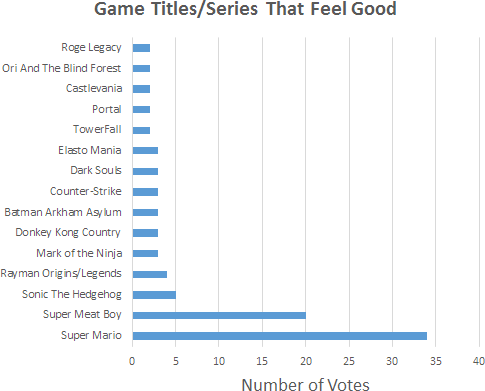
\includegraphics[width=0.9\columnwidth]{Pics/good_games}
%\caption{Game titles/series that the participants though feel good. Only those with more than one %vote are included.}
%\label{fig:good_games}
%\end{figure}

%\begin{table} \centering
%\caption{The 30 most commonly-used words to define game feel in general. Numbers in parenthesis %indicate usage frequency. Common grammar words have been excluded. Words with duplicate entries such %as \textit{games} and \textit{game} have been combined into one.}
%\label{table:mostWordsPost_GF}
%\begin{tabular}{lll}
%\toprule
%game (193) & feel (160) & control (87)\\
%how (46) & like (42) & player (34)\\
%good (26) & way (23) & character (22)\\
%really (18) & too (18) & something (17)\\
%should (17) & me (17) & play (16)\\
%gameplay (13) & responsive (13) & don't (13 times)\\
%get (13) & question (12) & easy (11)\\
%world (11) & bad (11) & responsiveness (11)\\
%will (11) & between (10) & actions (10)\\
%time (10) & important (10) & playing (9)\\
%\bottomrule
%\end{tabular}
%\end{table}

%\begin{table} \centering
%\caption{The 30 most commonly-used words to describe six other platform games in the post-questionnaire. Numbers in parenthesis indicate usage frequency. Common grammar words have been excluded. Words with duplicate entries such as \textit{games} and \textit{game} have been combined into one.}
%\label{table:mostWordsPost}
%\begin{tabular}{lll}
%\toprule
%game (252) & feel (214) & control (209)\\
%very (134) & played (97) & responsive (85)\\
%like (81) & jump (63) & never (58)\\
%fast (57) & character (57) & good (56)\\
%really (53) & mario (51) & great (50)\\
%slow (49) & floaty (47) & because (46)\\
%time (46) & too (45) & fun (45)\\
%just (43) & bit (42) & movement (41)\\
%precise (41) & hard (41) & super (40)\\
%jumping (40) & jumps (36) & frustrating (35)\\
%\bottomrule
%\end{tabular}
%\end{table}

%Figure \ref{fig:whatChanged} shows what the participants thought had changed between the rounds. Even though only acceleration and deceleration changed, participants also perceived other changes as well, most notably changes about how the controls felt in the air, such as how gravity and jumping worked. This might partially be due to the variable jump that some players may have missed in the first few rounds. Some also focused on the ball's properties, such as its mass and how ``ball-like" it behaved. 

%Participants were also asked to describe the feel of six platforming games. Below are some selected quotes for describing the feel of each (some quotes have been combined for the sake of clarity).

%\textbf{Mega Man (1987)}
%\vspace{-5mm}
%\begin{itemize}[noitemsep,nolistsep]
%\item Very slow and floaty. However, the game is based around moving slowly and attacking from a distance. The jumping is floaty, yet responsive to player inputs, such as changing direction in midair, or stopping the jump early. 
%\item Some jumps require pixel-perfect positioning, which makes you think actively about mechanics.
%\item Responsive, since Mega Man moves when you press the button, and stops when you don't.
%\item Very solid ground and air control. You have proper air control and Mega Man doesn't stop at the exact moment you let go of the D-pad. He slides a few pixels further, which feels natural.
%\item Super tight, super retro, no wiggle room.
%\end{itemize}

%\textbf{LittleBigPlanet (2008)}
%\vspace{-5mm}
%\begin{itemize}[noitemsep,nolistsep]
%\item Incredibly floaty to the point where it just isn't enjoyable. It feels like you have NO control %over the character.
%\item Nice and fluid. Sort of ``organic".
%\item Just terrible to control. Everything about the controls is too floaty, making precise jumping a %chore. A lot could have been improved by enabling D-pad controls, as the analog sticks tend to increase the floaty feel, and it's generally much more imprecise for this type of game.
%\item Game is very responsive but the control schemes are convoluted and overly complicated. 
%\item The slightly imprecise nature of the platforming makes for interesting mistakes to occur when playing with friends, but it is not so egregious that it is game breaking. 
%\item Child-like. Super happy. The animations really make a huge difference in how this game feels.
%\end{itemize}

%\textbf{Donkey Kong (1981)}
%\vspace{-5mm}
%\begin{itemize}[noitemsep,nolistsep]
%\item A bit sluggish, lends either a feeling of panic or frustration to me depending on whether I win or lose. Mario feels a bit difficult to control, the jumps are hard to gauge and he never seems to move quite quickly enough. It feels like slogging through a chest-high swamp.
%\item Good decent controls. It's very precise with no room for errors. But completely lacks any kind of air control.
%\item Precise and sloppy. Two words wide from each other, but it's the best I can describe it. It requires precision to jump the barrels, and the controls and overall feel provides that, but in the same time, it doesn't feel like you got much else control of Mario.
%\end{itemize}

%\textbf{Super Meat Boy (2010)}
%\vspace{-5mm}
%\begin{itemize}[noitemsep,nolistsep]
%\item Smooth and fast-paced movement that requires skill. Very good acceleration and deceleration of the character. 
%\item Fluid, precise, controlled, reactive, tight, streamlined, energetic.
%\item Massively floaty. The controls are often hailed as "tight", but that only seems to come from the responsiveness, not the actual movement physics, which are very floaty and unpredictable.
%\item Part of the game feel is sound design. In Meat Boy, you see him run up to speed, and as he gets faster you hear his little wet footsteps. It's rewarding to the player to get that feedback, it makes you FEEL fast. If Meat Boy was a red featureless square with no sound, it'd be a vastly inferior `feeling' game.
%\end{itemize}

%\textbf{Prince of Persia (1989)}
%\vspace{-5mm}
%\begin{itemize}[noitemsep,nolistsep]
%\item Static. The controls are very difficult to master because when you stop pressing a button the prince will still be moving, and therefore it is very hard to time you jump.
%\item Controls are responsive, but the movement is completely unpredictable due to the environment seemingly actually affecting the velocity and acceleration of the character.
%\item Tight, and yet a good sense of weight behind the character. Adventurous. Unforgiving, slippery.
%\end{itemize}

%\textbf{Super Mario Bros. (1985)}
%\vspace{-5mm}
%\begin{itemize}[noitemsep,nolistsep]
%\item It feels very responsive. Actions are quick and takes zero effort to master.
%\item The movement is a bit clunky, since Mario slides around, but it's okay, since the game doesn't have many big precise jumps.
%\item Floaty, awkward jumping and running. Momentum really holds and it feels like you are piloting a brick.
%\item Tight, predictable acceleration and momentum velocities. Instantly responsive controls, and although the character portrays a lot of acceleration and momentum after having stopped, it's always the same, becoming predictable and, thus, enjoyable.
%\item The run button pretty much allowed you to switch between two separate feels, one slow and one fast.
%\item Slow to accelerate, but the levels are designed around it. Top speed is fast, jump arc is nice.
%\end{itemize}

%As the above quotes illustrate, players tend to focus on different elements when it comes to game feel. What feels `unresponsive' and `floaty' to some may feel more responsive and relaxing to others. It all depends on the context of use, as one participant expressed when describing the feel of \textit{LittleBigPlanet}. If playing in a casual/social setting, it might not matter that the feel is `floaty' and `imprecise': \textit{``The slightly imprecise nature of the platforming makes for interesting mistakes to occur when playing with friends"}. It all comes down to what type of game it is and how challenging it's supposed to be. For instance, one participant described the feel of \textit{Super Mario Bros.} to be `clunky', but found it acceptable, since the game doesn't feature many big and precise jumps.